\section{Methodology}
\label{sec:methodology}

We started from a lexical baseline based on Apache Lucene BM25 and progressively moved to a multi-stage neural pipeline.
\newline
The final pipeline (Figure~\ref{fig:pipeline}) for the proposed information retrieval system, consists of four stages:
\begin{itemize}
    \item \textbf{Query translation}: queries in French or German are first translated into English.
    \item \textbf{Query expansion}: queries are expanded with additional context.
    \item \textbf{Retrieval}: relevant documents are retrieved from the corpus using the expanded query.
    \item \textbf{Reranking}: the retrieved documents are reranked based on their relevance to the original query.
\end{itemize}

\begin{figure}[htbp]
    \centering
    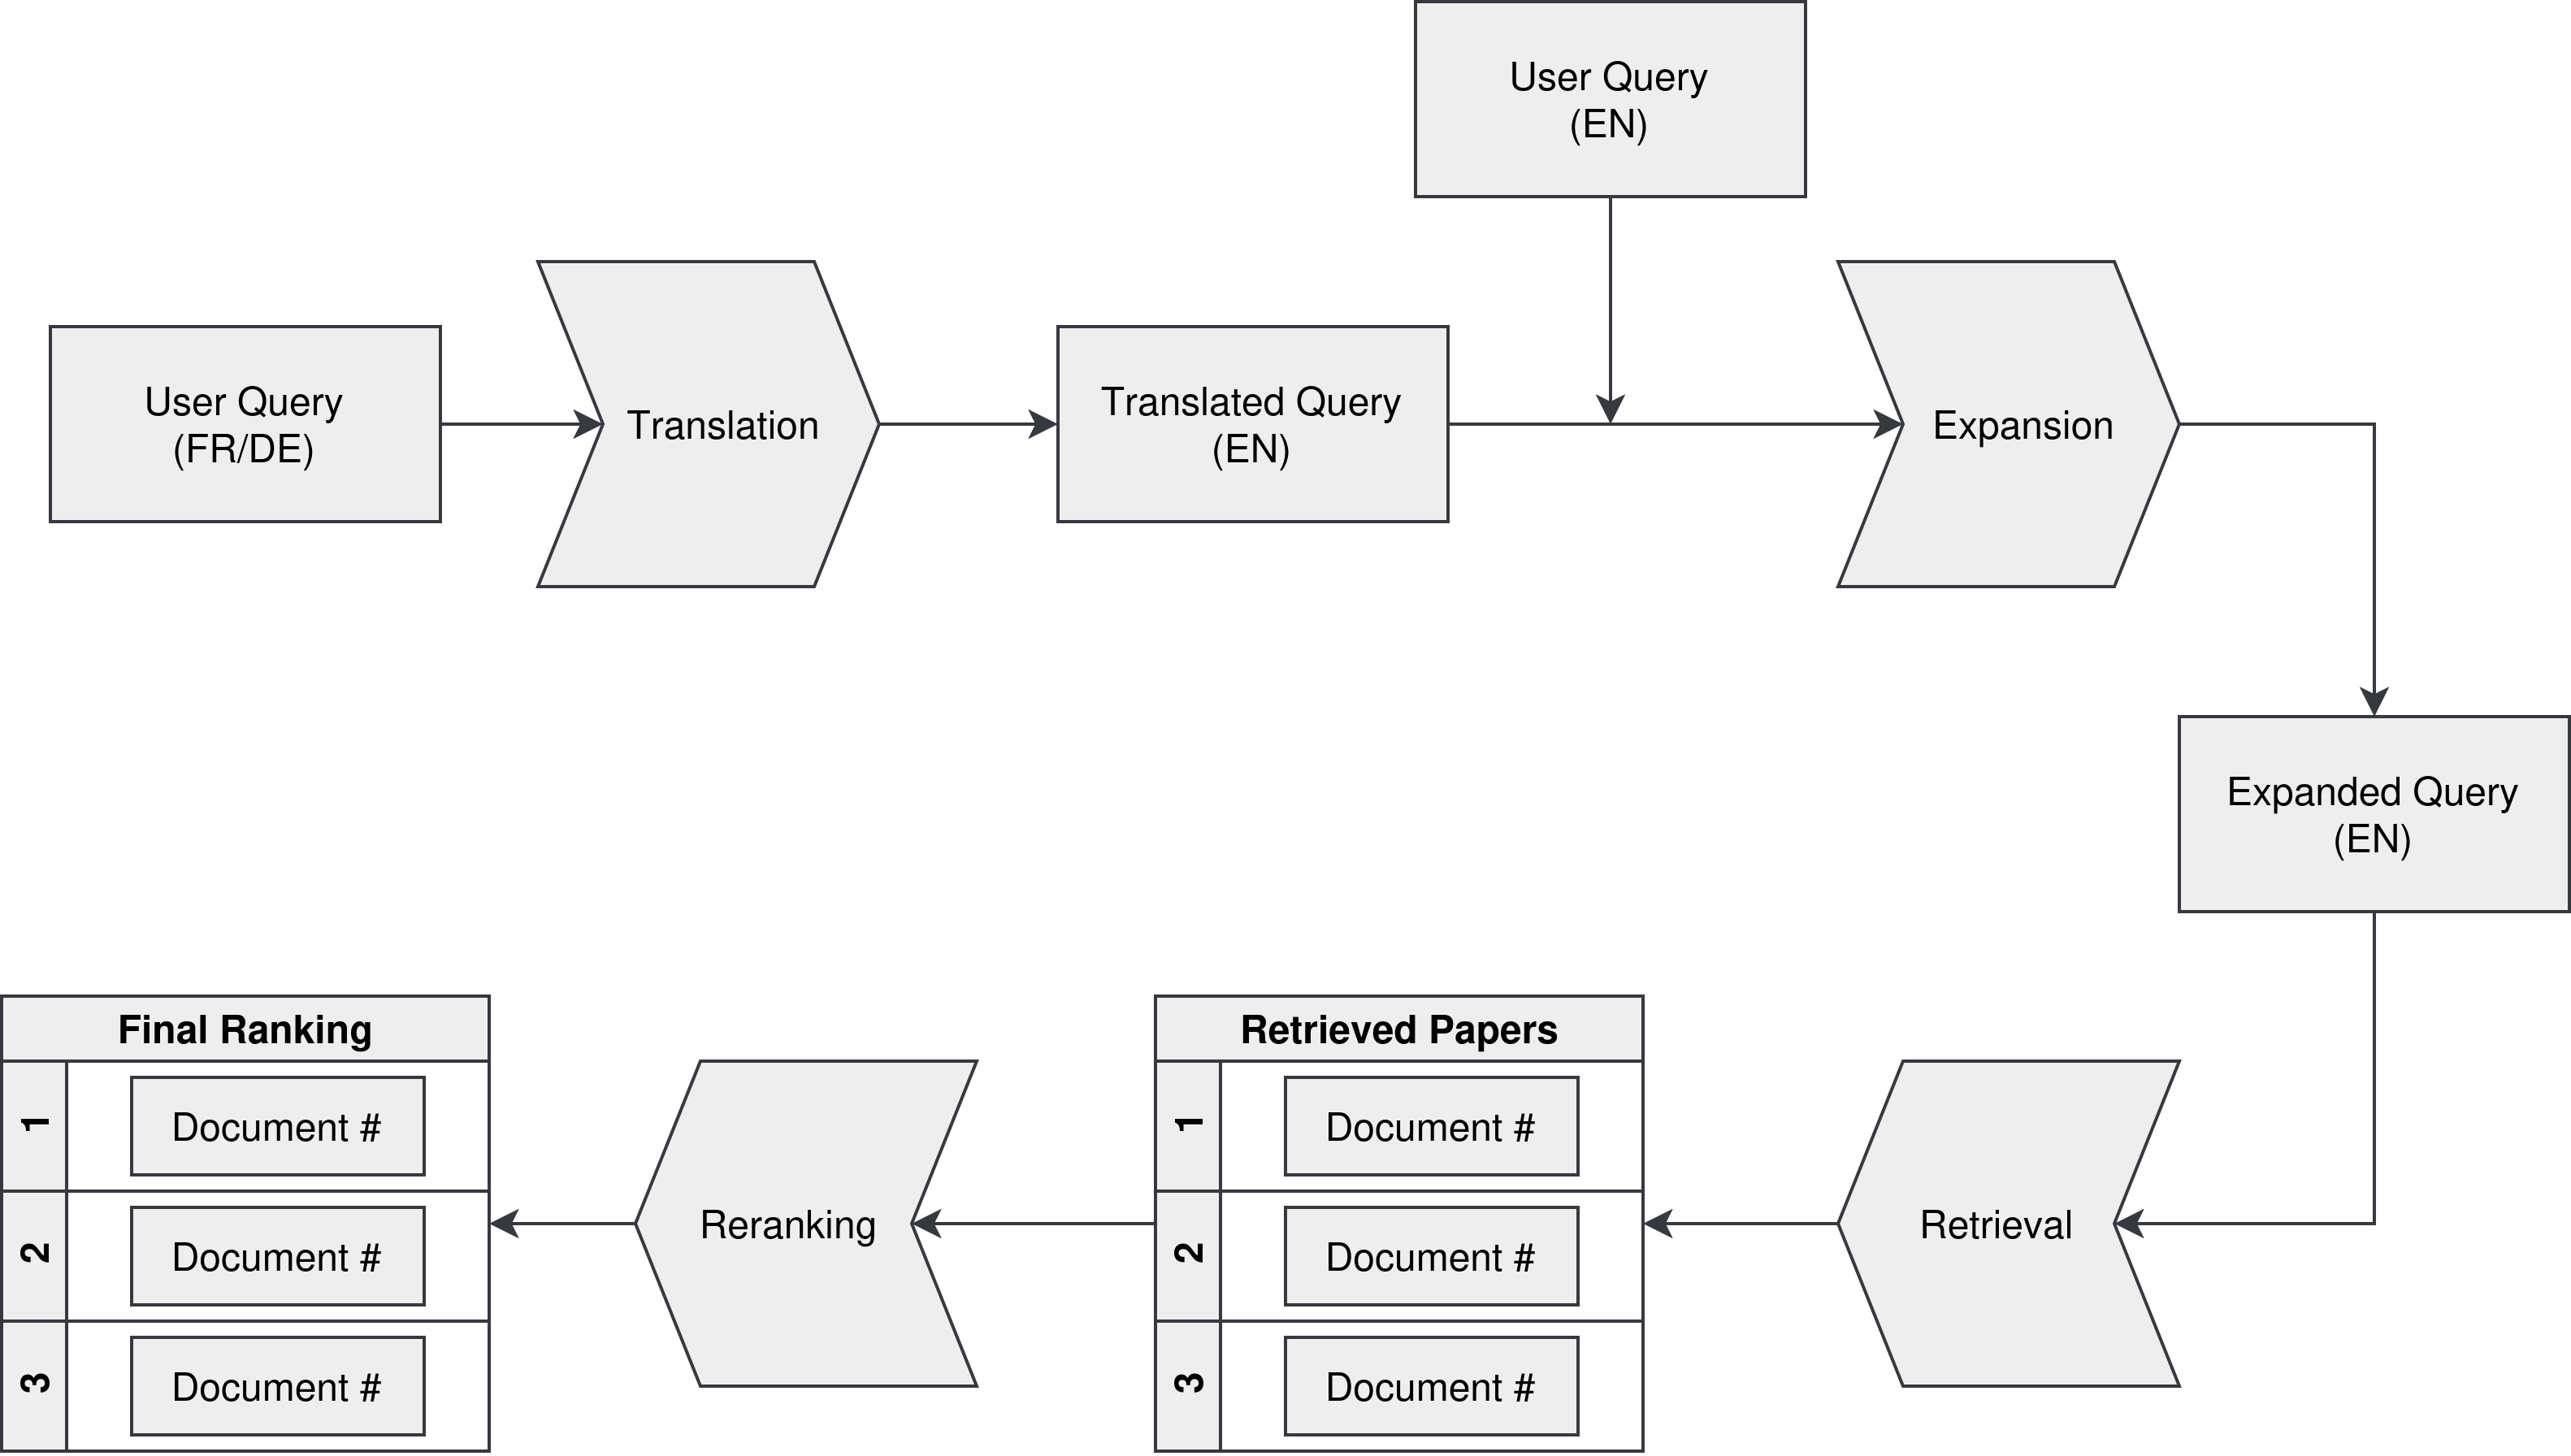
\includegraphics[width=0.8\linewidth]{figure/pipe.png}
    \caption{Four-stage pipeline for information retrieval.}
    \label{fig:pipeline}
\end{figure}

\subsection{Query translation} \label{sub:querytransl}
In the preliminary stage of our pipeline, non-English queries (French and German) are translated into English. This is done query by query using the model utter-project/EuroLLM-9B-Instruct-2512 with the following prompt:

\begin{promptbox}
    \small
    \ttfamily
    \begin{flushleft}
        \textit{system:} You are a professional translator.\\
        Translate the user's text to English.\\
        Output ONLY the English translation.\\
        Do not include the original text, explanations, labels, or any other content.\\[0.8em]

        \textit{user:} Translate this \{\textbf{French/German}\} text to English.\\
        Output only the English translation, nothing else.\\[0.8em]

        \{\textbf{Query original text $x$}\}
    \end{flushleft}
\end{promptbox}
Given $x$ as the original query text, the model predicts probabilities for the next token with \cite{huggingface_transformers_generation}:
$$P(y_t=i\mid y_{<t},x)=\operatorname{softmax}(z_t/T)_i$$
With our model configuration, the prediction becomes greedy, following \cite{utter_project_eurollm_9b_instruct_2512}: $$y_t=\arg\max_i P(y_t=i\mid y_{<t},x)$$
The resulting English queries are then fed into the following step of our pipeline.

\subsection{Query Expansion} \label{sub:query-expansion}

Following the translation stage, each query is processed by a deterministic query-expansion module designed to reduce query–document vocabulary mismatch between short user claims and the terminology used in the scientific corpus. The module does not rely on generative LLM-based paraphrasing. Instead, it combines lexical feature extraction with dense semantic retrieval and neighborhood-based term induction. 

\begin{itemize}
    \item The translated English query is first analyzed with spaCy’s en\_core\_web\_sm pipeline, which provides token-level linguistic annotations, including stop-word indicators and coarse-grained part-of-speech labels from the Universal POS tag set. Candidate lexical anchors are then identified by retaining tokens tagged as NOUN or PROPN while excluding stop words and tokens shorter than three characters. The resulting set is deduplicated to produce a compact lexical signature that captures the principal nominal content of the query.

    \item The semantic expansion stage operates over a corpus in which each document is represented as the concatenation of its title and abstract. These title–abstract pairs are embedded with BAAI/bge-large-en-v1.5. In accordance with the documented BGE retrieval interface \cite{bge-large-en-v1.5}, query embeddings are produced by prepending the instruction "\emph{Represent this sentence for searching relevant passages:}" to the translated query, whereas the corpus documents are encoded as retrieval targets. Similarity is then computed on normalized embeddings using the dot product. For unit-length vectors, dot-product scoring is equivalent to cosine similarity while being computationally more efficient.
    $$s(q,d)=e_q^\top e_d=\sum_i e_{q,i}e_{d,i}$$
    Because embeddings \(e = \frac{v}{\lVert v\rVert_2}\) are L2-normalized \(e_q^\top e_d = \cos(q,d)\) \cite{bge_large_model_card}.\\
    The five highest-scoring documents are retained as the local semantic neighborhood used for expansion.

    In the described implementation, candidate expansion terms are extracted from the retrieved documents after lowercasing, ASCII normalization, mention's and hashtag's symbols removal, stop-word filtering and exclusion of short tokens (tokens <= 2 characters long are discarded). The candidate pool is aggregated across the retrieved neighborhood and assigned weights derived from the semantic similarity of the source documents so that terms originating from more similar neighbors contribute more strongly. Terms already present in the query are removed and the fifteen highest-ranking candidates are retained as explicit expansion terms.
    \[
        K=\operatorname{unique}\{\ell(t): POS(t)\in\{\mathrm{NOUN},\mathrm{PROPN}\},\neg stop(t), |t|>2\}
    \]
    \[
        w_h=\max(1,\operatorname{round}(5s_h))
    \]
    \[
        c(t)=\sum_h w_h\,tf(t,d_h)
    \]
\end{itemize}
The final expanded query is constructed by concatenating three components: the cleaned (already translated) query, the noun and proper-noun-based keyword set extracted directly from the query and the expansion terms induced from the retrieved document neighbourhood.
This output expanded query is then used by the downstream retrieval pipeline.


\subsection{Retrieval} \label{sub:retrieval}
The retrieval stage is designed as a high-recall candidate-generation step between query expansion and neural reranking. Its objective is not to make the final relevance decision but to ensure that the true source paper is included in a sufficiently large candidate set for the subsequent, more computationally expensive cross-encoder stage. For this reason, after experimenting with a Lucene BM25 baseline, the final pipeline adopts BAAI/bge-m3 in a hybrid retrieval setting.

The retriever searches the fixed paper collection provided by the task organizers. Each paper is represented at document level by concatenating its title and abstract (batch size = 1024) and the retrieved unit is always the paper pubkey. Although the collection includes metadata such as venue and authors, this hybrid retrieval stage uses only titles and abstracts to speed up the inference time.

We chose BAAI/bge-m3 because it is well suited to this retrieval setting. The model can produce dense vectors, sparse lexical weights and ColBERT-style multi-vector representations from the same encoder.

This allows the retriever to combine broad semantic matching, exact term evidence and fine-grained token-level matching without switching between unrelated encoders.

For the dense representation, the document or query embedding is obtained from the normalized
CLS representation \cite{bge-m3}:
\[
    e=\operatorname{norm}(H[0])
\]
For the sparse representation, BGE-M3 assigns lexical weights to tokens \cite{bge_m3_docs}:
\[
    w_{qt}=\operatorname{ReLU}(W_{lex}^\top H_q[i])
\]
The sparse similarity between a query and a paper is then computed over overlapping terms:
\[
    s_{lex}=\sum_{t\in q\cap p} w_{qt}w_{pt}
\]

Candidate selection is performed in two steps. First, all documents are encoded as dense BGE-M3 vectors and searched with an inner-product FAISS index~\cite{faiss_documentation}.
The dense FAISS score is computed using inner product \cite{faiss_metrics}:
\[
    s_{IP}(q,d)=q^\top d
\]

Since the dense vectors are normalized, this inner product is equivalent to cosine similarity:
\[
    q^\top d=\cos(q,d)
\]
This dense stage acts as an efficient broad filter over the whole collection. The default setting retrieves a large candidate pool of \emph{candidate\_multiplier $\times$ top\_k}, with candidate\_multiplier = 3 and top\_k = 2000, before the final truncation.
The number of candidates passed to the hybrid rescoring stage is:
\[
    K_c=\min(N,\max(K,Km))
\]

This deliberately large candidate set favours recall, which is more important than precision at this stage.

Second, the dense candidates are rescored using the sparse and ColBERT-style representations. The sparse component rewards important overlapping terms, while the ColBERT-style component captures local token correspondences that may be lost when each document is represented by a single dense vector \cite{khattab2020colbert}.
The ColBERT-style late-interaction score is computed as \cite{khattab2020colbert}:
\[
    s_{colbert}(q,d)=\frac{1}{N_q}\sum_{i=1}^{N_q}\max_{1\le j\le N_d} q_i^\top d_j
\]

The final configuration was selected through a series of development runs. We first tuned the lexical baseline by varying the Lucene analyzer, stop-word lists, stemming strategy and BM25 searcher variants. These experiments improved the classical baseline but also highlighted its limitations for this task: even with query expansion and reranking, BM25-based candidate generation remained more dependent on surface-level lexical overlap than desired.

We also tested BGE-M3 in a hybrid retrieval setting, using a setup that differed slightly from the final configuration. In those experiments, sparse, dense and ColBERT-style retrieval were performed using dedicated query expansions tailored to each retrieval mode. More specifically, each query was represented through three complementary views: an embedding view for semantic matching, a sparse view for lexical and term-based evidence, and a ColBERT view for fine-grained token-level interaction.

However, the best results in our analysis were obtained with a simpler configuration in which BGE-M3 hybrid retrieval used the same expanded query, described in the previous section, for all three retrieval modes. We then tested several weighting configurations. Among them, the run labelled bge\_m3\_hybrid\_513 was retained because it provided the strongest recall-oriented trade-off among the retrievers evaluated without reranking. This configuration used weights of $0.5$, $0.15$ and $0.35$ for dense, sparse, and ColBERT scoring, respectively, with a multiplier of $3$ and a maximum hybrid input length of $384$.

A closely related configuration with a larger ColBERT weight achieved a nearly identical MRR@5 but a lower Recall@100. We therefore preferred the configuration that better matched the role of retrieval as a candidate generator. This choice was further confirmed by downstream experiments: reranking candidates from bge\_m3\_hybrid\_513 consistently outperformed the corresponding BM25-based reranked runs. In addition, increasing the reranked candidate depth from a few hundred documents to between $1000$ and $2500$ documents increased the final recall by giving the neural reranker a larger candidate pool.

The final hybrid retrieval score is therefore computed as:
\[
    s(q, d) =
    0.5\,s_{\text{dense}}(q, d)
    + 0.15\,s_{\text{sparse}}(q, d)
    + 0.35\,s_{\text{colbert}}(q, d).
\]

The largest weight is assigned to the dense score because it provides the main semantic signal. The sparse and ColBERT components add complementary lexical and fine-grained matching evidence. Candidates are sorted by this score in descending order and truncated to the final top\_k. The retrieval output is a JSON mapping each query ID to an ordered list of paper pubkeys.


\subsection{Reranking} \label{sub:reranking}
\subsubsection{Cross-encoder scoring}
Some rerankers have been tested:
\begin{itemize}
    \item Qwen/Qwen3-Reranker-4B \cite{qwen3embedding};
    \item Alibaba-NLP/gte-reranker-modernbert-base \cite{zhang2024mgte, li2023towards};
    \item nvidia/llama-nemotron-rerank-1b-v2\cite{llama-nemotron-rerank-1b-v2}.
\end{itemize}
 
From our findings, the strongest reranker is nvidia/llama-nemotron-rerank-1b-v2, a 1B-parameter LLaMA-based model fine-tuned as a sequence classifier. For each query-document pair, we build an input sequence using the official NVIDIA prompt template:
\begin{promptbox}
    \small\ttfamily
    question:\{query\} \textbackslash n \textbackslash n passage:\{passage\}
\end{promptbox}
The model computes a scalar logit $z \in \mathbb{R}$ through a linear classification head applied to the final hidden state and the relevance score is obtained by applying a sigmoid:
\[
    s(q, d) = \sigma(z) = \frac{1}{1 + e^{-z}}
\]
Documents are then sorted in descending order of $s(q, d)$.
Reranking deeper candidate pools (500-2500 documents) consistently produced better final results than shallower pools, confirming the importance of high recall at the retrieval stage to compensate for miss-labeling from weaker previous retrieval-stages and the reranker's ability to distinguish noise from documents that are actually relevant. 

At this stage, queries are evaluated against the corpus of the documents taking into account the title, abstract and author of the documents.

\subsection{Fine-tuning the Reranker} \label{sub:finetuning}
To improve the Nemotron reranker on the domain-specific characteristics of the CheckThat! task, we fine-tuned nvidia/llama-nemotron-rerank-1b-v2 using Parameter-Efficient Fine-Tuning (PEFT) with Low-Rank Adaptation (LoRA) on data from both the 2025 and 2026 editions of the task.

\subsubsection{Training data and hard-negative mining}
Training examples are query-document pairs with binary labels: a positive document is the gold source paper associated with the query while negative documents are hard negatives mined using sentence-transformers/static-retrieval-mrl-en-v1 \cite{static-retrieval-mrl-en-v1, reimers-2019-sentence-bert, kusupati2024matryoshka}. Hard negatives are selected from the range $[5, 50]$ nearest neighbors (by embedding similarity) that satisfy $\text{score} \leq 0.85$ and lie at least $0.05$ below the positive score in cosine similarity (absolute margin) preventing trivially easy or falsely relevant negatives from polluting training that would under-mine the effectiveness of the fine-tuning.

Training data combines two years of the task:
\begin{itemize}
    \item en\_train.json of the CheckThat! Lab CLEF 2026: split 90\% training / 10\% development. The development set is drawn exclusively from 2026 data for consistency with the official CT26 Task~1 evaluation protocol. Due to time-constraints and resource-constraints we used just the en\_train.json dataset but we suppose that also German and French translated queries datasets could improve the quality of the fine-tuning;
    \item All the datasets of task4/subtask\_4b, CheckThat! Lab CLEF 2025: all available topics (dev, test\_gold and train splits) are used entirely for training.
    
\end{itemize}
This design ensures that the dev set used to track MRR@5 during training is distribution-aligned with the contest test queries. Each training record contains one query, one positive passage and up to five hard negatives.

\subsubsection{LoRA architecture}
To fine-tune the 1B-parameter base model with limited GPU memory, we apply LoRA~\cite{hu2022lora} with rank $r = 16$ and scaling factor $\alpha = 32$. Adapters are inserted into all attention and feed-forward projection layers:
q\_proj, k\_proj, v\_proj, o\_proj, gate\_proj, up\_proj and down\_proj.
The classification head (score) is included in
modules\_to\_save and is fully updated during training. The task type is SEQ\_CLS, matching the sequence-classification objective of the reranker.

\subsubsection{Training objective}
The model produces a single scalar logit $z$ per input pair.
Training minimizes binary cross-entropy with logits over all
positive ($y=1$) and negative ($y=0$) pairs in each batch:
\[
    \mathcal{L} = -\frac{1}{B}\sum_{i=1}^{B}
    \Bigl[ y_i \log \sigma(z_i) + (1 - y_i)\log(1 - \sigma(z_i)) \Bigr]
\]
where $B$ is the effective batch size and $\sigma$ is the sigmoid function. Gradient accumulation over 4 steps is used to simulate a larger effective batch size of 32 without additional memory overhead.

\subsubsection{Optimization}
The model is trained with AdamW, a learning rate of $2 \times 10^{-5}$, a linear warmup over 10\% of the total training steps and gradient clipping at norm 1.0. Training runs for 3 epochs with bfloat16 mixed precision and gradient checkpointing enabled to reduce VRAM usage. The checkpoint with the best MRR@5 on the 2026 development set is retained.

\subsubsection{Inference}
At inference time, the LoRA adapter weights are merged into the base model via merge\_and\_unload() before scoring, so no PEFT overhead is incurred during evaluation. The scoring procedure and prompt format are identical to those of the base reranker (Section~\ref{sub:reranking}) and the fine-tuned model is used as a drop-in replacement in the reranking stage.

\subsection{Evaluation}
We evaluate systems on the CheckThat! Task 1 query sets by matching retrieved pubkeys against the gold pubkey for each query. The official evaluation metric for the task is MRR@5. We also tracked Recall@100 to monitor candidate-generation quality and to verify that reranking gains do not come from overly aggressive filtering.
\clearpage